\documentclass[doktyp=semarbeit, sprache=german]{TUBAFarbeiten}
\usepackage[utf8]{inputenc}
\usepackage[T1]{fontenc}
\usepackage{graphicx} 
\usepackage{amsmath}
\usepackage{subcaption}
\usepackage{booktabs}
\usepackage{url}
\usepackage{listings}
\usepackage{color}

\definecolor{dkgreen}{rgb}{0,0.6,0}
\definecolor{gray}{rgb}{0.5,0.5,0.5}
\definecolor{mauve}{rgb}{0.58,0,0.82}

\lstset{frame=tb,
	language=C++,
	aboveskip=3mm,
	belowskip=3mm,
	showstringspaces=false,
	columns=flexible,
	basicstyle={\small\ttfamily},
	numbers=none,
	numberstyle=\tiny\color{gray},
	keywordstyle=\color{blue},
	commentstyle=\color{dkgreen},
	stringstyle=\color{mauve},
	breaklines=true,
	breakatwhitespace=true,
	tabsize=3
}
\captionsetup{compatibility=false}
\bibliographystyle{unsrt}
\TUBAFFakultaet{Fakultät für Maschinenbau, Verfahrens- und Energietechnik}
\TUBAFInstitut{Institut für Automatisierungstechnik}
\TUBAFTitel[Moderne Methoden der Bildverarbeitung am Beispiel Gesichtserkennung]{Moderne Methoden der Bildverarbeitung am Beispiel Gesichtserkennung}
\TUBAFUntertitel{Anwendung von Informations- und Automatisierungssystemen}
\TUBAFBetreuer{Prof. Andreas Rehkopf}
\TUBAFAutor[S. Dressel und H. Krumbiegel]{Samuel Dressel und Hannes Krumbiegel}
\TUBAFDatum{\today}
\begin{document}
\maketitle
\tableofcontents
\newpage
\section{Einleitung}
Wenn man von Automatisierungssystemen redet, so erstreckt sich der Anwendungsbereich von diesen Systemen längst nicht nur auf den industriell-technischen Sektor. Vielmehr kommen diese Systeme grade im Zug der Digitalisierung auch in völlig neuen Anwendungsgebieten zum Tragen. Dazu gehören auch Systeme, die es ermöglichen, Gesichter zu erkennen und zu identifizieren.
Der Einsatzspektrum dieser Technik reicht dabei vom automatischen Toilettenpapierspender bis hin zum bargeldlosen Bezahlen mittels Gesichts-ID. Grade in den letzten Jahren wurden hier neue Methoden und Technologien entwickelt, welche die Verwendung solcher Systeme immer effizienter und kostengünstiger machen. Dazu gehören vor allem neue Forschungserkenntnisse im Bereich des maschinellen Lernens und die steigende Rechenleistung von Computertechnik. Dies erlaubt es, unterschiedlichste Prozesse in der Industrie und Dienstleistung zu optimieren und wichtige Ressourcen einzusparen.
\\\\In dieser Arbeit soll ein grober Überblick über verschiedene Techniken und Methoden der Gesichtserkennung und -identifizierung gegeben werden. Dabei wird in Kapitel \ref{sec:grundlagen} zunächst auf einige wichtige Grundlagen eingegangen; in Kapitel 3 und 4 jeweils die zwei Teilbereiche Gesichtserkennung und Gesichtsidentifizierung näher beleuchtet und in Kapitel 5 eine Zusammenfassung gegeben. 
\section{Grundlagen}
\label{sec:grundlagen}
Einführend zum besseren Verständnis des Themenkomplexes ist es wichtig, einige wesentliche Begriffe zu definieren und außerdem voneinander abzugrenzen. Dabei gilt es, zwischen der Lokalisation eines Gesichtes an sich und der Zuordnung des Gesichts zu einer bestimmten Person zu unterscheiden. Im ersten Fall wird geprüft, ob und wo ein Gesicht zu sehen ist, im zweiten, um wen es sich handelt \cite{FaceRecognitionWikipedia}. Wir sprechen somit zum einen von der Gesichtserkennung und zum anderen von der Gesichtsidentifizierung. Im englischen Sprachgebrauch unterteilt man den Teil der Gesichtsidentifizierung zusätzlich noch in eine menschliche Erkennung (\textit{face perception}) und in eine maschinelle Erkennung (\textit{face recognition}). In dieser Arbeit wird sich jedoch lediglich auf die maschinelle Gesichtsidentifizierung beschränkt.
\newpage

\section{Gesichtserkennung (Face Detection)}

Verschiedene Methoden können verwendet werden, um zu entscheiden, ob ein Bild ein Gesicht enthält. Die Möglichkeiten beinhalten u. a. neuronale Netze, genetische Algorithmen oder speziell für das Problem entwickelte Lösungsansätze. Die Gesichtserkennung ist ein rechnerisch einfacheres Problem als die in Kapitel \ref{identifizierung} behandelte Gesichtsidentifizierung; allerdings besteht beispielsweise bei Fotokameras der Wunsch, auf wenig leistungsfähigen Prozessoren die Aufgabe in Echtzeit durchzuführen, um einen schnellen Fokus auf die Gesichter zu ermöglichen. Dieser Anwendungsfall erfordert einen möglichst effizienten Algorithmus.  

Der folgende Abschnitt soll einen kurzen Abriss über die verschiedenen Möglichkeiten der Gesichtserkennung geben und exemplarisch einen besonders effizienten Vertreter, den 2001 von Viola und Jones veröffentlichten Viola-Jones-Algorithmus, im Detail vorstellen \cite{Viola01rapidobject}.

\subsection{Genetische Algorithmen}
Wong, Lam und Sui entwickelten einen genetischen Algorithmus, der mögliche Gesichtskandidaten als Chromosomen auffasst und die Evolution imitiert, um ein Gesicht zu finden \cite{WONG20011993}. Die Fitness eines Chromosoms beschreibt, wie sehr es einem Gesicht ähnelt. Chromosomen mit einer hohen Fitness behält der Algorithmus (\glqq Selektion\grqq) und modifiziert sie durch von der Natur inspirierten Rekombinations- und Mutationsoperatoren. Diese Schritte wiederholt er mehrere Generationen lang, um letztendlich die besten Gesichtskandidaten zu erhalten.

\subsection{Neuronale Netzwerke}
Neuronale Netzwerke, darunter insbesondere Convolutional Neural Networks, eignen sich gut für viele Aufgaben des maschinellen Sehens. Neben Objekterkennung und Gesichtsidentifizierung befindet sich darunter auch Gesichtserkennung. Valliant et al. entwickelten schon 1994 einen Algorithmus, der Gesichter mithilfe von neuronalen Netzwerken erkennt \cite{Object}.

\subsection{Viola-Jones-Algorithmus}
Der Viola-Jones-Algorithmus ist ein häufig zur Gesichtserkennung eingesetzter Algorithmus. Er verarbeitet in Graustufen umgewandelte Bildausschnitte und nutzt sogenannte \textit{Haar-like-Features}, schwarz-weiße Rechteckanordnungen, um in den Ausschnitten Gesichter zu identifizieren. Diesen Prozess optimiert er mithilfe von verschiedenen Techniken, z. B. den des Integralbilds und einer Attention-Kaskade. Das Resultat ist ein effizienter Algorithmus, der sich auch von schwachen Rechnern in Echtzeit berechnen lässt.

\subsubsection{Vorverarbeitung}
Der Viola-Jones-Algorithmus operiert ausschließlich auf der Grundlage von Graustufenbildern, weshalb der er im ersten Schritt Farbbilder in diese umwandelt.

Der zweite Schritt dient dazu, die Geschwindigkeit des Algorithmus zu erhöhen. Ein Bild, das weniger Pixel enthält, kann schneller verarbeitet werden, weshalb das Herunterskalieren des Bildes die Performance erhöht. Sehr kleine Gesichter können durch die Reduktion der Auflösung verloren gehen, aber in Anwendungsfällen, wo dies akzeptabel ist, ist der Schritt sinnvoll.

Der dritte Schritt besteht darin, iterativ alle möglichen Bildausschnitte auszuwählen, die ein Gesicht enthalten könnten und demzufolge von einem Gesichtserkennungs-Unteralgorithmus darauf überprüft werden sollen. Es ist beispielsweise möglich, dass das gegebene Bild eine einzige Großaufnahme eines Gesichts ist, der gesuchte Bildausschnitt betrifft hier das ganze Bild. In anderen Fällen enthält ein Bild viele kleine Gesichter: Um diese zu finden, muss der Algorithmus alle Bildausschnitte, die so groß sind wie die gesuchten Gesichter, überprüfen. Letztendlich überprüft der Algorithmus alle Bildausschnitte vorher festgelegter Größen, die von sehr groß bis klein variieren.

\subsubsection{Haar-like-Features}
\begin{figure}
	\centering
	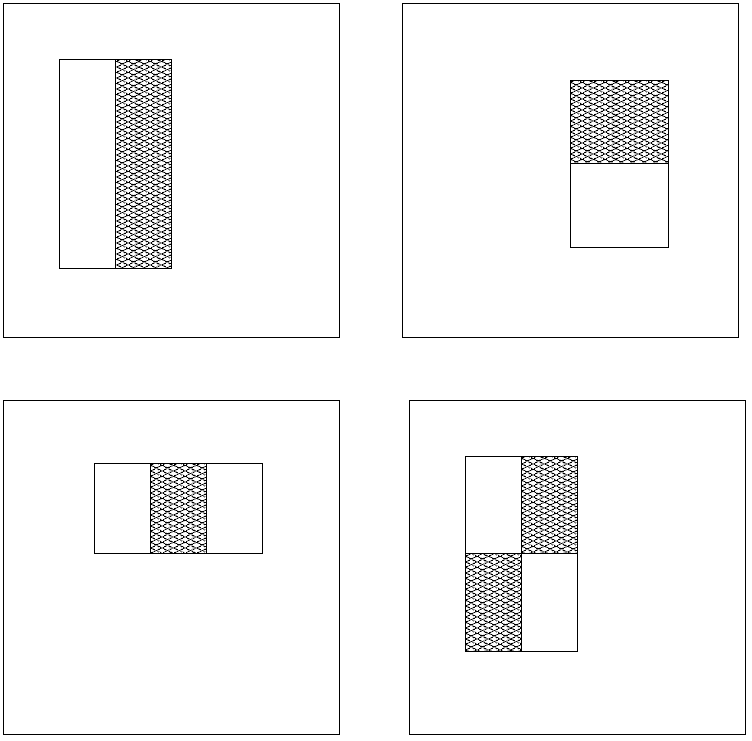
\includegraphics[width=0.4\linewidth]{images/haarfeatures}
	\caption[Haar-like-Features]{Mehrere mögliche Haar-like-Features. Quelle: \cite{Viola01rapidobject}}
	\label{fig:haarfeatures}
\end{figure}


Ein Haar-like-Feature besteht aus mehreren schwarzen oder weißen Rechtecken und hat das Ziel, markante dunkle bzw. helle Teile eines Gesichts abstrakt abzubilden. Der Wert eines solchen Features beschreibt, wie gut es auf einen Teil eines Graustufenbildes passt.

Ein Feature, das aus einem schwarzen Rechteck über einem weißen Rechteck besteht, wird einen hohen Wert haben, wenn das schwarze Rechteck über die Augenpartie und das weiße über Nase und Wangen gelegt wird (siehe Abbildung \ref{fig:haarfeatures2}). Bei Teilen des Bildes, die kein Gesicht enthalten, ist dies selten der Fall. Bei einem Bildausschnitt, bei dem viele - für die Gesichtserkennung ausgewählte - Features hohe Werte aufweisen, handelt es sich wahrscheinlich um ein Gesicht.

\begin{figure}
	\centering
	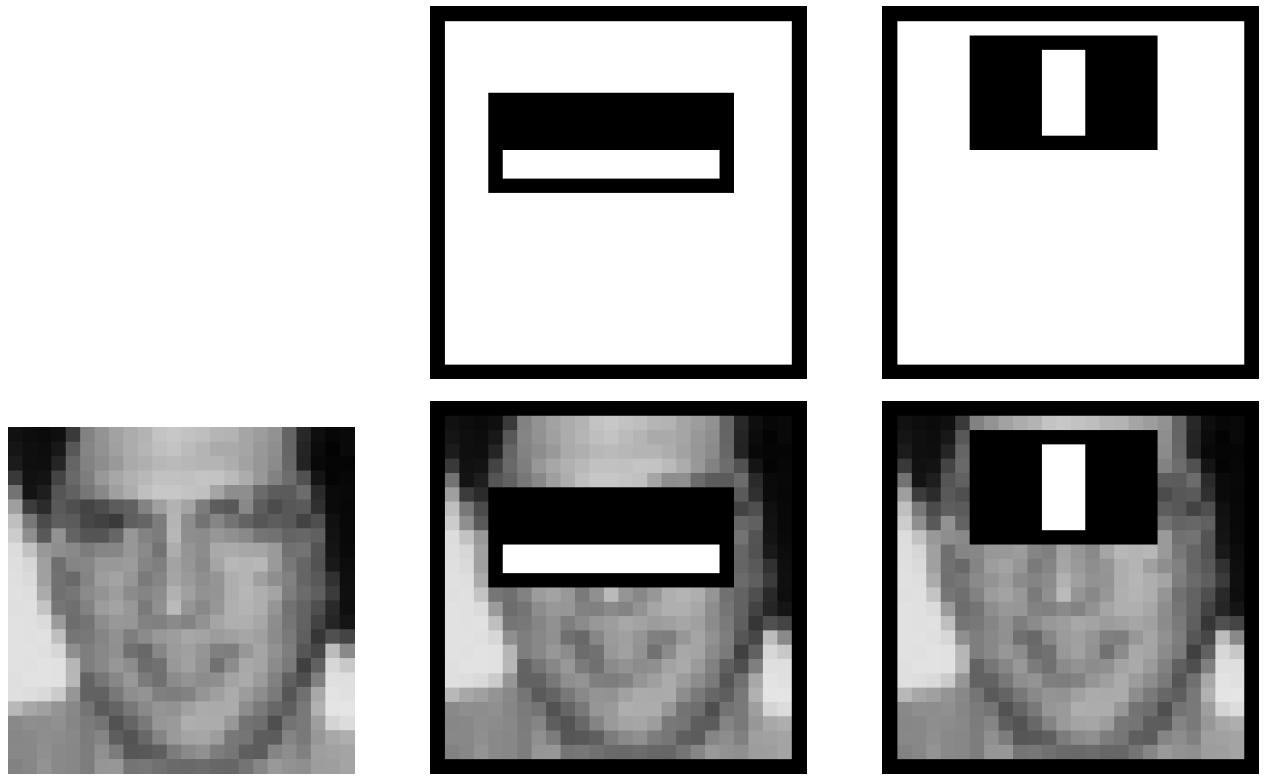
\includegraphics[width=0.7\linewidth]{images/haarfeatures2}
	\caption[Haar-like-Features - Beispiel]{Zwei Haar-like-Features, die ein Gesicht sehr gut beschreiben. Quelle: \cite{Viola01rapidobject}}
	\label{fig:haarfeatures2}
\end{figure}

Der Wert eines solchen Features berechnet sich aus der Summe der Helligkeitswerte der Pixel unter dem schwarzen Rechteck(en), von denen die Summe der Helligkeitswerte unter den weißen Rechteck(en) abgezogen wird. Ein weißes Pixel hat einen Helligkeitswert von 0, ein schwarzes Pixel entspricht dem Wert 255. Ein Feature erreicht dementsprechend seinen Maximalwert, wenn unter seinen weißen Rechtecken nur weiße Pixel und unter seinen schwarzen Rechtecken nur schwarze Pixel liegen.

\subsubsection{Integralbilder}

\begin{figure}
	\centering
	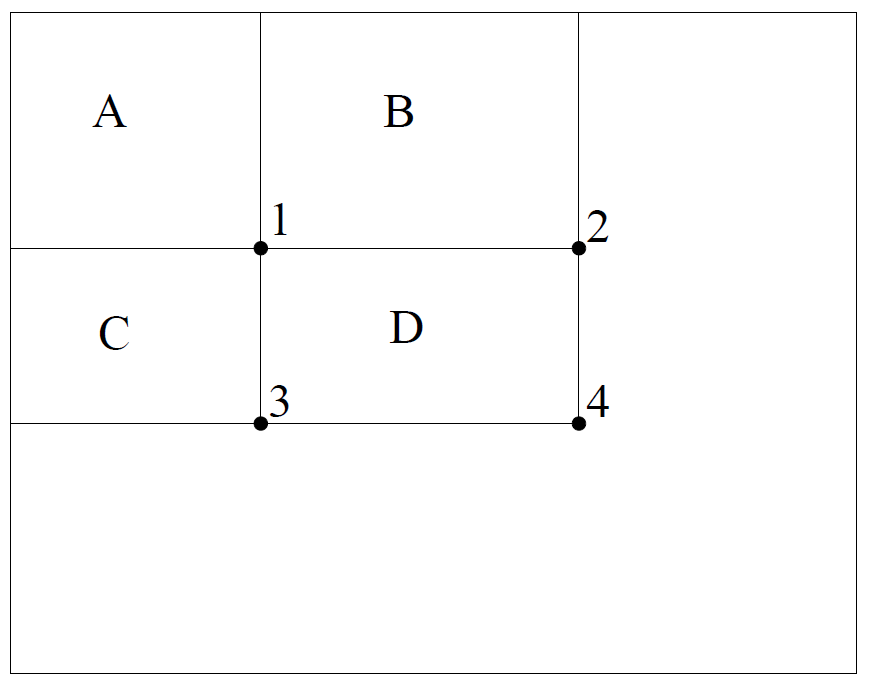
\includegraphics[width=0.7\linewidth]{images/integral}
	\caption[Integralbild]{Eine Illustration eines Integralbildes. Quelle: \cite{Viola01rapidobject}}
	\label{fig:integral}
\end{figure}


Während des Viola-Jones-Algorithmus müssen die Werte von sehr vielen Haar-like-Features berechnet werden. Eine einfache Implementierung für die Berechnung des Werts eines weißen oder schwarzen Rechtecks bestünde aus einer doppelten For-Schleife, die zwischen den Grenzen der x- bzw. y-Achse iteriert und alle Pixelwerte aufaddiert. Ein Rechteck der Dimension 10x10 würde somit 99 Additionen erfordern.

Viola und Jones entwickelten in \cite{Viola01rapidobject} das Konzept des Integralbilds, das es ermöglicht, die Anzahl der Rechenoperationen stark zu reduzieren. Das Integralbild ist eine Matrix, die an der Position jedes Pixels des Bildes nicht den Wert des Pixels, sondern die Summe aller Pixelwerte speichert, die links oberhalb des Pixels liegen. Abbildung \ref{fig:integral} verdeutlicht dies: Der Eintrag an Position 1 speichert z. B. die Summe der Pixel der Fläche A.

Das Integralbild ermöglicht es, die Summe der Pixel in einem beliebigen Rechteck nur durch 3 Rechenoperationen zu ermitteln. Die Abbildung verdeutlicht dies: Der Eintrag an Position 4 speichert die Summe der Pixel der Flächen A + B + C + D. Wenn wir die Summe der Pixel der Fläche D ermitteln möchten, können wir von dem Wert die Einträge 2 (entspricht d. Summe von A + B) und 3 (entspricht d. Summe von A + C) subtrahieren. Zuletzt müssen wir lediglich den Flächeninhalt von A - gespeichert in Matrixeintrag 1 - wieder addieren, da er im vorherigen Schritt doppelt subtrahiert wurde. 

Der Algorithmus berechnet das Integralbild einmal pro Bild und kann es dann für jedes Haar-like-Feature in jedem Bildausschnitt wiederverwenden.

\subsubsection{Feature-Auswahl}
Viola und Jones verwenden in ihrer Implementierung Bildausschnitte der Größe 24 x 24 Pixel \cite{Viola01rapidobject}. Schon bei dieser relative geringen Auflösung existieren über 160000 verschiedene mögliche Features. Mithilfe einer Gesichtsdatenbank kann ein Brute-Force-Algorithmus bestimmen, welche dieser Features Gesichter am besten von anderen Objekten unterscheiden können. Die Features mit den höchsten Klassifizierungsgenauigkeiten zeigt Abbildung \ref{fig:haarfeatures2}. Dennoch haben auch sie eine Fehlerrate von über 10 Prozent. Um hohe Genauigkeiten zu erreichen, müssen mehrere Features kombiniert werden.

Ein einfacher Ansatz wäre es, für die Klassifizierung die Werte der \textit{n} besten Features für jeden Bildausschnitt zu berechnen. Dies führt jedoch nicht zu optimalen Ergebnissen, da z. B. die Kombination zweier sehr ähnlicher Features, die in den gleichen Fällen ein vorhandenes Gesicht nicht erkennen, zu keiner Verbesserung führt. Viola und Jones haben sich hier für den AdaBoost-Algorithmus für die Featureauswahl entschieden. Dieser wählt Features sukzessive aus und bevorzugt dabei Features, die Gesichter korrekt klassifizieren, welche von den bisher ausgewählten Features falsch klassifiziert werden.

\subsubsection{Kaskade}
\begin{figure}
	\centering
	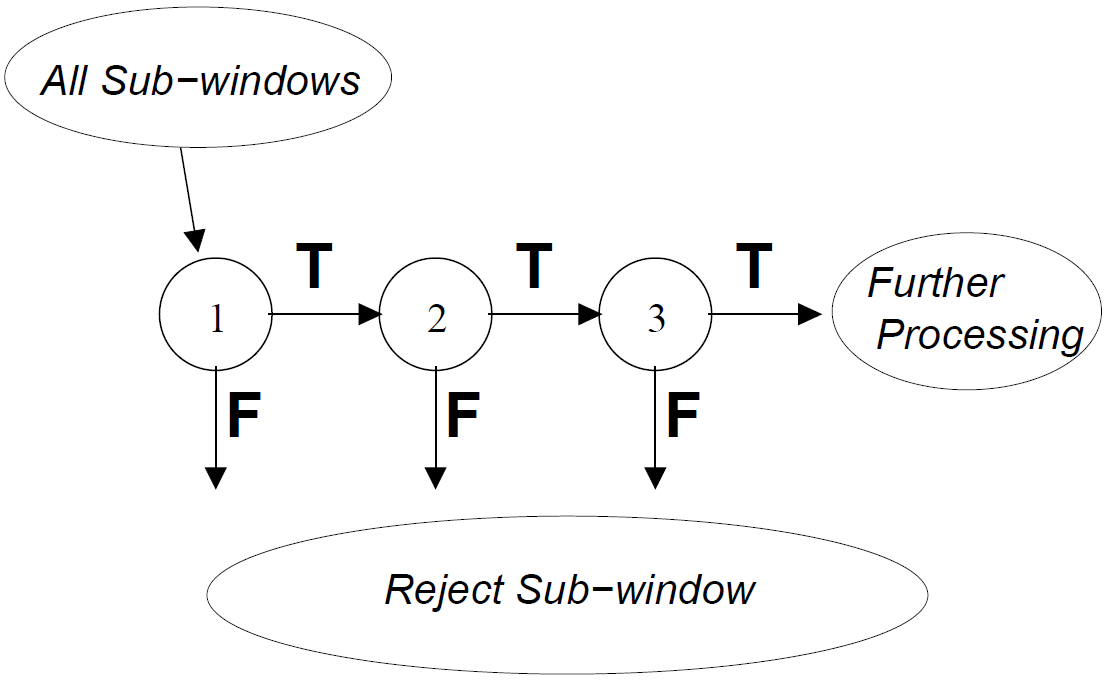
\includegraphics[width=0.7\linewidth]{images/cascade}
	\caption[Kaskade]{Eine sogenannte Kaskade, ein Entscheidungsbaum, der Bildausschnitte ohne Gesicht schnell aussortieren soll. Quelle: \cite{Viola01rapidobject}}
	\label{fig:cascade}
\end{figure}


Von allen Bildausschnitten, die der Algorithmus auf ein vorhandenes Gesicht prüft, enthalten die meisten keine Gesichter. Um endgültig zu mit hoher Genauigkeit verifizieren, ob ein Ausschnitt ein Gesicht enthält, benötigt der Algorithmus Tausende Features.

Damit er nicht alle Features berechnen muss, um offensichtliche Ausschnitte ohne Gesicht auszusortieren, verwenden Viola und Jones eine sogenannte \textit{Kaskade} \cite{Viola01rapidobject}. Dieser Ansatz verbessert die Performance erheblich und wird in neueren Arbeiten auch bei der Gesichtserkennung ohne Haar-like-Features verwendet \cite{Li_2015_CVPR}.

Eine Kaskade besteht aus mehreren Stufen: Jeder Bildausschnitt muss alle Stufen klassifizieren, um als Gesicht erkannt zu werden. Wenn eine Stufe erkennt, dass ein Ausschnitt sicher kein Gesicht ist, wird dieser aussortiert. Viola und Jones setzten in ihrer Implementierung eine erste Stufe ein, die nur aus zwei Features besteht und 100 Prozent aller Gesichter durchlässt, aber in der Lage ist, 60 Prozent aller Nicht-Gesichter auszusortieren.

\subsubsection{Nachverarbeitung}

Falls das Bild ein Gesicht enthält, werden einige der Bildausschnitte die Kaskade vollständig durchlaufen und als Gesicht erkannt. Häufig erkennt der Algorithmus mehrere sich stark überschneidende Ausschnitte als zwei separate Gesichter. Der letzte Schritt besteht darin, diese wieder zusammenzuführen.

\subsubsection{Verwendung des Algorithmus unter Nutzung von OpenCV}
Es ist nicht einfach, einen effizienten Viola-Jones-Algorithmus zu implementieren. Dazu sollte der Programmierer nicht nur den Algorithmus verstehen, sondern auch Technologien wie SIMD oder CUDA. Für Entwickler, die lediglich an den Resultaten des Algorithmus interessiert sind, bietet sich die Verwendung einer schon vorhandenen Implementierung an.

Eine Bibliothek, die den Algorithmus implementiert, ist OpenCV \cite{opencv_library}. Optional bietet sie CUDA-Unterstützung an, wobei der Großteil des Algorithmus auf der Grafikkarte und nicht auf dem CPU abläuft.

OpenCV erfordert nur wenige Schritte für die Ausführung des Viola-Jones-Algorithmus. Die Bibliothek stellt vorgefertigte Kaskaden in der Form von XML-Dateien zur Verfügung und implementiert den Algorithmus in nur einer Funktion. Der folgende Codeblock zeigt in leicht gekürzter Form die Anwendung der Bibliothek.

\begin{lstlisting}
CascadeClassifier face_cascade; //Initialisiert ueber XML-Datei
Mat picture; //Bild, in dem Gesichter erkannt werden sollen. (Initialisiert in nicht gezeigtem Code.)
Mat picture_gray;

cvtColor(picture, picture_gray, COLOR_BGR2GRAY); //Wandle Bild in Graustufen um
std::vector<Rect> faces;
face_cascade.detectMultiScale(frame_gray, faces); //Fuehrt den Viola-Jones-Algorithmus aus und speichert die Resultate in der Variable "faces"
\end{lstlisting}


\section{Gesichtsidentifizierung (Face Recognition)}
\label{identifizierung}
Das Gebiet der Gesichtsidentifizierung umfasst alle Methoden und Techniken, mit der es möglich ist, basierend auf visuellen Material Menschen eindeutig zu identifizieren. Die Gesichtsidentifizierung baut dabei auf der Gesichtserkennung auf. Insbesondere in den letzten Jahren wurden nach und nach zahlreichen Algorithmen und Methodiken entwickelt, um Gesichter maschinell zu identifizieren. Insbesondere im Hinblick auf die Automatisierung der Gesichtsidentifizierung stellt erst das Jahr 1973 den Startpunkt dar, als Takeo Kanade in seiner Dissertation das erste automatisierte System zur Gesichtsidentifizierung vorstellte \cite{Takeo}. Jedoch konnte grade aufgrund der begrenzten Rechenleistung zu dieser Zeit dieses System noch längst nicht effizient arbeiten. Ein wesentlicher Fortschritt wurde erst im Jahr 1990 durch die Forscher Kirby und Sirovich erzielt, welche die Hauptkomponentenanalyse (Karhunen-Loève-Transformation) verwendeten \cite{Kirby}. Hierbei wird eine Vielzahl von generierten Variablen auf eine geringe Zahl aussagekräftiger Parameter reduziert. Dadurch wird gleichzeitig auch die Komplexität und der Rechenaufwand verringert. Weiterhin stellte die Arbeit von Matthew Turk und Alex Pentland einen weiteren Meilenstein dar, welche sogenannte Eigengesichter (Eigenvektoren) zur Gesichtsidentifizierung nutzten \cite{Turk}. Diese Techniken werden auch noch in den derzeitigen State-of-the-Art-Methoden genutzt.
\\\\Im Folgenden soll auf eine Reihe dieser Methoden und Herangehensweisen eingegangen, einige Anwendungsbeispiele genannt und die Problematiken der Gesichtsidentifizierung thematisiert werden.
\subsection{Methoden der Gesichtserkennung}
Grundlegend können alle Methoden der Gesichtsidentifizierung in zwei wesentliche Schritte eingeteilt werden. Der erste Schritt ist die Extraktion und Selektion von Merkmalen aus dem visuellen Input; der zweite Schritt stellt die Klassifizierung der Merkmale dar \cite{FRS}. Desweiteren können Techniken zur Gesichtsidentifizierung in die Art der verwendeten Merkmale unterteilt werden. Diese können entweder geometrische Features (Form der Augen, Position der Nase, ...) oder fotometrische Features sein (Texturen, Farbwerte, ...).
\begin{figure}
	\centering
	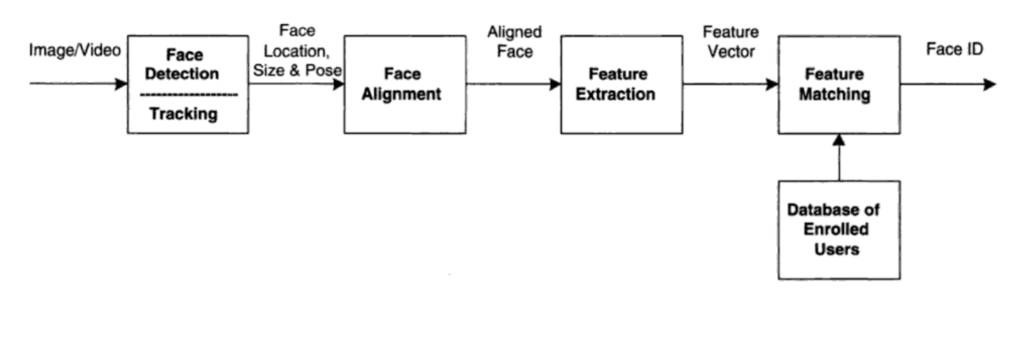
\includegraphics[width=1\textwidth]{images/process}
	\caption{Verallgemeinerte Darstellung des Gesichtsidentifzierungsprozessen als Prozessbild \cite{DeepLearning}}
	\label{img:process}
\end{figure}
\\Die obenstehende Abbildung \ref{img:process} gibt einen grafischen Überblick über den Prozess der Gesichtsidentifzierung. Zunächst wird durch Gesichtserkennung nach einem Gesicht in dem vorhandenen Video- bzw. Bildmaterial gesucht (\textit{Face Detection}). Dann wird das Bild durch bestimmte Bildmanipulationsmethoden in eine zur weiteren Verarbeitung nutzbare Form gebracht (\textit{Face Alignment}). Dies umfasst unter anderem Transformationen (Drehung, Neigung, ...) und die Veränderung von Helligkeits- und Kontrastwerten. In dem folgenden Schritt werden dann die benötigten Features für die jeweilige Gesichtsidentifizierungsmethode extrahiert, selektiert und klassifziert (\textit{Feature Extraction}). Diese werden dann mit einer vorhandenen Datenbank abgeglichen und führen letztendlich zum Identifizierungsergebnis (\textit{Feature Matching}).
\subsubsection{Hauptkomponentenanalyse (PCA) mit Eigengesichtern}
Das erste Verfahren, welches im Rahmen dieser Ausarbeitung näher betrachtet werden soll, ist die Hauptkomponentenanalyse (Principal Component Analysis, PCA) mit Eigengesichtern. Die Idee der Gesichtsidentifizierung mit PCA ist es, vorhandenes Bildmaterial so zu reduzieren, dass es sich für eine Auswertung eignet, ohne dabei die wesentlichen Merkmalsinformationen zu verlieren \cite{PCANova}. Man spricht hier von einer Dimensionsreduzierung. Die Hauptkomponentenanalyse an sich beinhaltet noch nicht den kompletten Prozess der Gesichtsidentifizierung, sondern stellt vielmehr ein Tool dar, welches von finalen Methoden im ersten Schritt der Selektion genutzt wird. Dies ist vor allem im Hinblick auf die Effizienz dieses Prozesses von großer Wichtigkeit.
\begin{figure}
\captionsetup[subfigure]{justification=centering}
\centering
\begin{subfigure}[c]{0.49\textwidth}
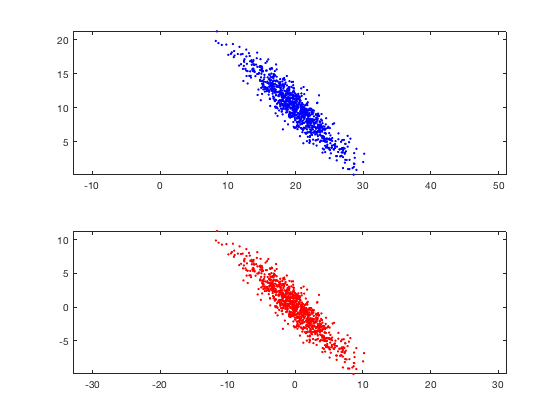
\includegraphics[width=1\textwidth]{images/PCA1.png}
\subcaption{Zweidimensionale Punktewolke - beide Datensätze sind identisch mit dem Unterschied, dass das rot gefärbte Diagramm nullzentriert ist}
\end{subfigure}
\begin{subfigure}[c]{0.49\textwidth}
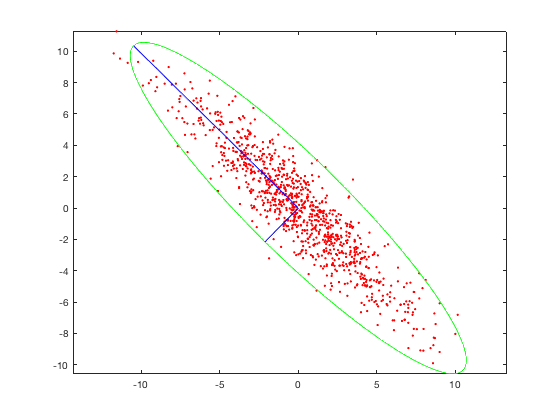
\includegraphics[width=1\textwidth]{images/PCA2.png}
\subcaption{Durch Bestimmung der Eigengesichter generierte Achsen; die längere der beiden blauen Achsen stellt dabei die Achse mit einer maximalen Streuung der Daten da, wenn die Punktewolke auf diese projiziert wird}
\end{subfigure}
\caption{Reduzierung der Dimension einer zweidimensionalen Punktewolke }
\label{img:PCA}
\end{figure}Um die Funktionsweise der Hauptkomponentenanalyse mit Eigengesichtern zu verstehen, kann man sich die einzelnen Merkmale als zweidimensionale Punktewolke vorstellen (Abbildung \ref{img:PCA}a). Eine Dimensionsreduzierung wird den Datensatz in diesen Fall von einer zweidimensionalen Ebene in eine eine eindimensionale Ebene transformieren \cite{PCAPython}. Wie auch bei allen anderen Algorithmen zur Dimensionsreduzierung geschieht dies im Fall der Hauptkomponenentenanalyse durch das Finden einer Hyperebene, auf welche die einzelnen Punkte projiziert werden können. Bei der Hauptkomponentenanalyse wird die Hyperebene so gewählt, dass bei einer Projektion alle Punkte eine maximale Streuung erzielen. Es wird sozusagen die Achse der maximalen Varianz gesucht. Im Fall der Punktewolke in Abbildung \ref{img:PCA} ist dies die längere blaue Linie. Um diese Linie zu finden, kommen nun die sogenannten Eigengesichter zum Tragen. Diese Eigengesichter sind nichts anderes als die Eigenvektoren der Kovarianzmatrix der gegebenen Datenmenge. Da in dem Fall der Hauptkomponentenanalyse die Achsen der maximalen Varianz generiert werden, bleiben die wichtigsten Informationen aus der Menge von Merkmalen erhalten. Für den zweiten Schritt der Klassifizierung im Rahmen der Gesichtsidentifizierung wirkt sich eine große Streuung zusätzlich positiv aus.
\subsubsection{Deep Learning}
Die meisten Merkmale, die bei einer Gesichtsidentifizierung durch einen Menschen offensichtlich sind, sind es für einen Computer nicht. Die einfachste Methode, um gewisse Merkmale eines Gesichtes für den Computer als \glqq wichtig\grqq{} zu markieren, ist eine eigenständige Abwägung des Computers in Hinblick auf die Wichtigkeit eines Merkmals. Dafür werden meist Methoden des maschinellem Lernens (Deep Learnings) genutzt. Die Methode des maschinellen Lernens kann für eine Vielzahl von Merkmalsformen genutzt werden wie unter anderem Wärmesignaturen, Gesichtsform oder Gesichtstextur \cite{DeepLearning}.
\subsubsection{Dreidimensionale Gesichtsidentifzierung}
Die dreidimensionale Methode der Gesichtsidentifzierung nutzt ein gewisses räumliches Sensorsystem, um Informationen zur Form des Kopfes zu generieren \cite{Drei}. Diese Informationen werden dann genutzt, um bestimmte Merkmale wie die Form und Kontur von Augen, Nase und Mund zur Identifizierung zu benutzen. Der große Vorteil dieser Technik ist, dass die Identifizierungsvorgang auch bei schlechten Lichtverhältnissen durchgeführt werden kann und einen größeren Spielraum hinsichtlich des Aufnahmewinkels besitzt. Der Nachteil dieser Methode ist die Fehleranfälligkeit von durch Mimik gezeigten Emotionen, welche die Form der einzelnen Gesichtsmerkmale verzerren.
\subsubsection{Gesichtstexturanalyse}
Ein viel genutzter Ansatz zur Gesichtsidentifizierung ist die sogenannte Gesichtstexturanalyse (\textit{Skin texture analysis}). Diese Methode extrahiert und nutzt die visuellen Details der Gesichtshaut \cite{SkinTexture}. Dabei wird ein aufgenommes Foto zunächst in einzelne Blöcke aufgeteilt. Diese Blöcke werden dann mit diversen Algorithmen in einen mathematischen Raum abgebildet. Diese extrahierten Daten können dann mit einem bestehenden Datensatz verglichen werden. Bei einer hinreichend guten Auflösung kann ein solches Gesichtsidentifizierungssystem selbst winzige Poren und Hautlinien erkennen kann. Tests mit diesen Systemen konnten sogar eineiige Zwillinge voneinander unterscheiden, was mit herkömmlichen Systemen meist nicht erreicht werden konnte. Besonders effektiv ist diese Methode der Gesichtsidentifzierung in Verbindung mit anderen Methoden der Gesichtsidentifzierung.
\subsubsection{Wärmebildverfahren}
Einen ganz anderen Ansatz als bisher vorgestellte Methoden zur Gesichtsidentifizierung bilden die Wärmebildverfahren \cite{Thermal}. Hier kommt der Input für den Identifkationsprozess von Wärmebildkameras. Dabei nehmen diese Kamers nur die Form und die Wärmesignatur des Kopfes auf und ignorieren dabei Accessoires wie Brillen, Kopfbedeckungen oder Makeup. Der Vorteil des Einsatzes einer Wärmebildkamera ist die Tatsache, dass die Bildaufnahme auch bei schlechten Lichtverhältnissen stattfinden kann; Bildaufnahmen bei Nacht inbegriffen. Der Nachteil des Einsatzes von Thermalbildern ist der limitierte Vergleichsdatensatz, der letztendlich für eine Identifikation notwendig ist.
\begin{figure}
	\centering
	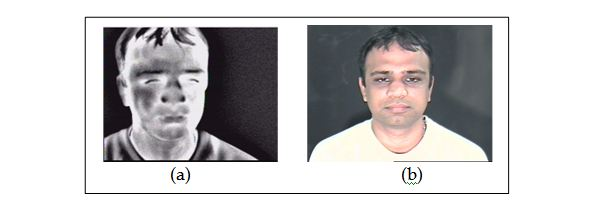
\includegraphics[width=1\textwidth]{images/thermal}
	\caption{Thermalbild eines Gesichts \cite{Thermal}}
	\label{img:thermal}
\end{figure}
2018 wurde von Forschern des U.S. Army Research Laboratory eine Technik entwickelt, die einen Vergleich von Wärmebildern mit Bildern einer herkömmlichen Kamera vergleichen kann. Umgesetzt wird dies wiederum durch die Verwendung von maschinellem Lernen. Dabei wird hier zunächst ein einzelnes Thermalbild synthetisiert indem verschiedene einzelne Gesichtsregionen und darin enthaltene Gesichtsdetails analysiert. Danach kann dieses Bild wiederum mit vorhandenen konventionellen Fotos innerhalb einer Personendatenbank verglichen werden \cite{Army}.
\subsection{Anwendung}
Mit den derzeitig vorhandenen Methoden und einer ausreichend hohen Rechenleistung lässt sich die automatisierte Gesichtsidentifizierung vielfältig nutzen und wird auch mehr und mehr in verschiedensten Anwendungsgebieten eingesetzt. Ein erstes großes Anwendungsgebiet ist sicherlich die Nutzung zu Überwachungszwecken und in Verifizierung von Personen in rechtstaatlichem Kontext. Dies geschieht grade in Staaten wie China, Russland oder der USA. Als Beispiel sei hier das \glqq Next Generation Identification System\grqq{} des FBI genannt, welches mit einer Genauigkeit von 85 \% Personen identifizieren kann \cite{FBI}. Weiterhin setzt China hier unter Verwendung von Künstlicher Intelligenz neue Maßstäbe im Hinblick auf eine totale Überwachung \cite{China}. Beispielsweise werden Bürger, die bei Rot über die Ampel gehen, durch Kameras identifiziert und durch Bildschirme öffentlich als Verkehrssünder angeprangert. Hier werden auch die negativen Aspekte des Einsatzes deutlich.
\\Weiteren Einsatz findet die Gesichtsidentifizierung auch privaten und finanziellen Sektor. Hier reicht die Einsatzreichweite von dem Entsperren von Türen und Smartphones bis hin zum Bezahlen mithilfe der Gesichts-ID.
Einen Meilenstein erzielte Facebook mit der Entwicklung von \glqq Deep Face\grqq{}, welches die Personenidentifzierung mit einer Genauigkeit von 97 \% erlaubt \cite{DeepFace}. Um diese Genauigkeit zu erzielen, wurde eine neurales Netz mit neun Schichten und 120 Millionen Gewichtungen benutzt und mithilfe von vier Millionen Facebook-Profilbildern trainiert.
\subsection{Kritik und Probleme}
Die Thematik der Gesichtsidentifizierung im Vergleich zu einer lediglichen Gesichtserkennung im Sinne der Unterscheidung von anderen Objekten bringt eine Vielzahl von neuen Problemen mit sich. Und dies längst nicht nur auf der technischen Seite, sondern auch im Hinblick auf ethische Aspekte.
Betrachtet man die auftretenden Probleme der technischen Umsetzung, so können unterschiedliche Herausforderungen durch die Verwendung von unterschiedlichen Methoden und Technologien gemeistert werden. Jedoch werden bestimmte Schwierigkeiten noch längst nicht vollständig gelöst. Klassische Methoden, welche ihren Input aus klassischem Bildmaterial beziehen, haben mit einer Reihe ganz unterschiedlicher Probleme zu kämpfen \cite{MainBook}:
\begin{itemize}
\item Viele zweidimensionale Methoden liefern nur verwendbare Ergebnisse unter ausreichend guten Lichtverhältnissen. Auch ein großer Kontrast bzw. Variation der Beleuchtung kann die Effizienz dieser Methoden erheblich einschränken.
\item Die Verdeckung insbesondere der oberen Gesichtsareale durch eventuelle Gadgets wie Brillen, Hüte oder Kapuzen verringert die Genauigkeit oder kann eine Gesichtsidentifizierung nahezu unmöglich machen. Abhilfe schafft hier die Verwendung von Wärmesignaturen zur Gesichtsidentifzierung.
\item Klassische Verfahren, die auf die Textur bzw. die Form des Gesichts zur Identifizierung angewiesen sind, funktionieren nur, wenn ein ausreichend optimaler Blickwinkel auf das Gesicht gegeben ist.
\item Bei der Identifizierung von Menschen muss der natürliche Alterungsprozess und damit die Veränderung des Gesichts als ein negativer Faktor beachtet werden. Dies erfordert entweder eine aktuelle Vergleichsdatenbank oder das Verwenden einer hinreichend guten KI, um den Alterungsprozess des Gesichts abbilden zu können.
\item Ein weiteres Problem im Hinblick auf eine fotometrische Gesichtserkennung sind Emotionen. Diese können ähnlich wie Verdeckungen durch eine damit einhergende Gesichtsverzerrung die Identifizierung wesentlich ungenauer machen.
\end{itemize}
Neben den technologischen Herausforderungen der Gesichtsidentifizierung ergeben sich auch eine Reihe von ethischen Problemen bzw. Kontroversen. Viele Menschenrechtsorganisationen und private Kampagnen zeigen immer wieder Zweifel und äußern Kritik, wenn es um den Einsatz dieser Technologien im Überwachungsbereich geht. Diese Bedenken reichen bis hin zum Gegenstand einer der \glqq totalen Überwachungsgesellschaft\grqq{}, bei dem Staaten und andere Autoritäten die Fähigkeit haben, die Überwachung ihrer Bürger umfassend auszuweiten. Die Verwendung von Identifizierungstools bietet außerdem Möglichkeiten des Missbrauchs im Hinblick auf die digitale Welt (Social Profiling \cite{SocialProfiling}).
\section{Zusammenfassung und Ausblick}
Die in dieser Arbeit vorgestellten Methoden und Techniken der Gesichtserkennung- und identifzierung bieten für eine Vielzahl von Problemen in unterschiedlichen Anwendungsbereichen hinreichend gute Lösungen. Die Anwendungsbereiche gehen dabei längst über die klassische Verwendung im Überwachungssektor hinaus. Vielmehr können durch neueste Methoden auch Bereiche wie der Forschungs-, Finanz- und Industriesektor bedient werden. In jedem Fall ist im Hinblick auf die Forschung noch längst nicht die Grenze des Möglichen erreicht. Mit der Entwicklung neuer Technologien in diesem Bereich werden gewisse Nachteile von bestehenden Ansätzen ausgeglichen, jedoch entstehen damit auch gleichzeitig neue Fragen grade was den ethischen Aspekt von der Gesichtsidentifizierung angeht. Hier gilt es, einen Einsatz immer Hinblick auf die Einschränkung der persönlichen Freiheit abzuwägen. Im Großen und Ganzen überwiegt trotzdem der Vorteil der Nutzung von Systemen zur Gesichtserkennung- und identifzierung: durch die Verwendung derselben können Zeit und Ressourcen gespart werden. Dafür stehen für verschiedene Einsatzzwecke unterschiedlichen Methoden bereit. Es bleibt nach wie vor spannend, wie die Entwicklung in diesem Bereich in den nächsten Jahren voranschreiten wird.
\newpage
\bibliography{literatur}{}
\addcontentsline{toc}{section}{Literatur} 
\end{document}